\chapter{Métodos de optimización} 
\label{chap:mopt}

    La optimización consiste buscar valores para un conjunto de parámetros que
ma\-xi\-mi\-cen o minimicen la función objetivo del problema tratado de modo que
se satisfagan las restricciones del mismo. Una solución factible es una
elección de valores para el conjunto de parámetros que satisfacen todas las
restricciones del problema. Las soluciones factibles con mejores valores de
función objetivo son llamadas soluciones óptimas.

Las técnicas de optimización son usadas diariamente para planificación
industrial, administración de recursos, programación de horarios, toma de
decisiones, reconocimiento de patrones, etc\cite{GO_1}. Por lo tanto, son
ampliamente usadas en muchos campos como ingeniería, industria, medicina y
negocios. La investigación en el campo de la optimización es bastante
activa y nuevos métodos son desarrollados regularmente \cite{GO_1}.

La optimización abarca tanto problemas de maximización como de minimización.
Cualquier pro\-ble\-ma de maximización puede ser convertido en un problema de
minimización al tomar la inversa de la función objetivo del mismo y
viceversa. En general, un problema de optimización puede ser definido como:

    Sea $S$ el espacio de soluciones y $d$ su dimensión donde:
\begin{itemize}
    \item $f: S \rightarrow \mathbb{R}$ es la función objetivo de minimización del problema.
    \item $S \subseteq \mathbb{R}^d$
\end{itemize}
    entonces se debe encontrar $x^* \in S$ tal que:
\begin{itemize}
    \item $f(x^*) \leq f(x), \forall x \in S$, si se desea tratar un problema de minimización.
    \item $f(x^*)^{-1} \geq f(x)^{-1}, \forall x \in S$, si se desea tratar un problema de maximización.
\end{itemize}

El valor de $f(x^*)$ (ó $f(x^*)^{-1}$) es llamado óptimo global. La
optimización global es la tarea de encontrar la solución óptima global. En
general, existen soluciones que son localmente óptimas, pero no globalmente
óptimas (ver figura \ref{mopt:maxmin}). Por lo tanto, los problemas de optimización
global son difíciles de resolver de manera exacta. En el contexto de problemas
combinatorios, estos problemas son frecuentemente \emph{NP-hard}\footnote{Un
problema es \emph{NP-hard} si todos los problemas en \emph{NP} se pueden reducir
a él en tiempo polinomial.\cite{NPHARD}} \cite{GO_2}. Un buen algoritmo de
optimización global encontrará $x^*$ sin importar el punto inicial $x_0 \in S$.

\begin{figure}[h!]
  \centering
  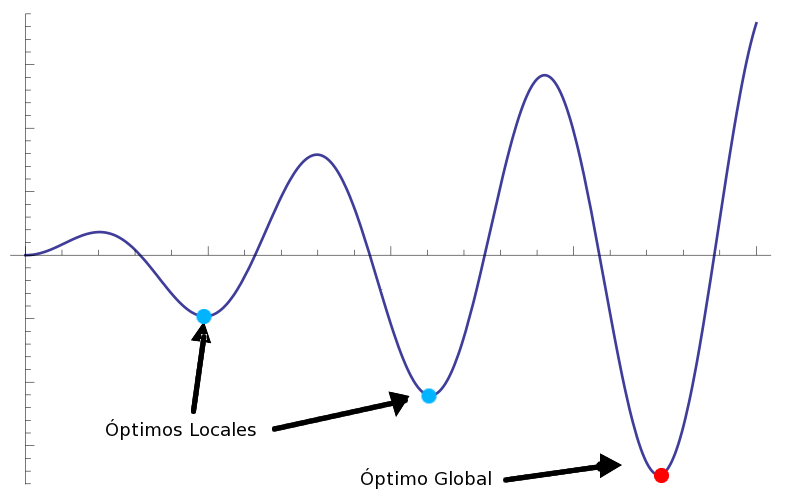
\includegraphics[width=0.5\textwidth]{figures/maxmin.png}
  \caption{Óptimos locales y globales para un problema de minimización}
  \label{mopt:maxmin}
\end{figure}

    Algunos ejemplos de problemas de optimización global son \cite{GO_2}:
\begin{itemize}
    \item Problemas combinatorios: donde la función lineal o no-lineal es definida
sobre un conjunto finito, pero muy grande, de soluciones. Por ejemplo, la
\textbf{agrupación no supervisada de datos}, la programación de horarios, entre
otros.
    \item Problemas generales sin restricciones: donde se define una función
no-lineal sobre un conjunto de valores reales sin restricciones.
    \item Problemas generales con restricciones: donde se define una función
no-lineal sobre un conjunto de valores reales con restricciones.
\end{itemize}

\subsection{Algoritmos tradicionales de optimización}

    Los algoritmos de optimización tradicionales usan métodos exactos para
encontrar la mejor solución. Si el problema tiene solución, entonces estos algoritmos
son capaces de encontrar la solución óptima global.

    Algunos de estos algoritmos son \cite{TA_1}:
\begin{itemize}
    \item \emph{Fuerza bruta}: comparan todas las soluciones del espacio de
soluciones, de modo que encontrar la solución óptima global esté garantizado. Sin
embargo, a medida que crece el espacio de soluciones, el costo de los algoritmos
de fuerza bruta incrementa. Por lo tanto, no son apropiados para la clase de
problemas pertenecientes al grupo \emph{NP-hard}.
    \item Programación lineal: sirven para problemas donde una variable depende
de una o más variables de manera lineal:
\begin{center}
    $f(X_1, X_2, \cdots, X_n) = a_1 \cdot X_1 + a_2 \cdot X_2 + \cdots + a_n \cdot X_n$
\end{center}

En otras palabras, $f(X_1, X_2, \cdots, X_n)$ (función objetivo del algoritmo)
puede ser expresada como una combinación lineal de las variables
$X_1, X_2, \cdots, X_n$. 
    \item Programación dinámica: funciona bajo el principio de encontrar una
solución total, operando en un punto intermedio que está entre la ubicación actual
y la ubicación final. El procedimiento es recursivo y cada punto intermedio es una
función de los puntos ya visitados. Una vez alcanzada la meta, se puede reconstruir
de manera inversa el camino óptimo generado por el algoritmo.
\end{itemize}

\subsection{Algoritmos Estocásticos}

Los algoritmos estocásticos son usados para hallar soluciones
cercanas al óptimo global para pro\-ble\-mas \emph{NP-hard} en tiempo polinomial. Estos
algoritmos logran su objetivo al suponer que las soluciones buenas están
cercanas unas de otras en el espacio de búsqueda. Sin embargo, a diferencia de
los algoritmos tradicionales, estos podrían no encontrar la solución óptima
global \cite{PSO_0}.

Los algoritmos estocásticos tienen varias ventajas comparados con otros
algoritmos \cite{SA_1}:
\begin{itemize}
    \item Son generalmente fáciles de implementar.
    \item Pueden ser usados eficientemente en paralelo.
    \item No requieren que la función de definición del problema sea continua.
    \item Generalmente pueden encontrar la solución óptima o cercana a la
óptima.
    \item Sirven para problemas discretos y combinatorios.
\end{itemize}

Algunos algoritmos estocásticos son \cite{PSO_0}:
\begin{itemize}
    \item \textbf{Hill-Climbing}: consiste en tomar una solución potencial
aleatoria del problema $x_0$ y buscar, en la vecindad $V_0$ de $x_0$, una nueva
mejor solución al problema. Si se encuentra una $x_1 \in V_0$ tal que $x_1$ es
mejor que $x_0$, entonces $x_1$ es la nueva solución potencial y se repite el
procedimiento que se hizo con $x_0$. Si no se encuentra una solución $x_1 \in V_0$
tal que $x_1$ es mejor que $x_0$, entonces $x_0$ es la mejor solución encontrada
por el algoritmo \cite{TA_1}.
    \item \textbf{Simulated Annealing}: consiste en tomar una solución aleatoria
del problema $x_0$ y un valor pequeño $\epsilon$ para perturbar las soluciones.
Si $x_0 + \epsilon$ es mejor que $x_0$, entonces la nueva mejor solución es 
$x_0 + \epsilon$ y se repite el procedimiento. Sino, la solución $x_0$ será
perturbada con una probabilidad que se va decrementando a medida que avanza la
ejecución del algoritmo \cite{SA_2}.
    \item \textbf{Búsqueda \emph{Tabú}}: consiste en una búsqueda heurística que
mantiene una lista de memoria \emph{tabú} de las soluciones previamente visitadas, de
modo que se mejore el proceso de búsqueda. La lista \emph{tabú} es usada como una guía
de movimiento de una solución a la siguiente para evitar ciclos \cite{SA_5} y que
se quede atrapado en un óptimo local. Inicialmente, \emph{Tabú} comienza su búsqueda
con una solución elegida aleatoriamente. A partir de la solución actual, se
generan un conjunto de soluciones de prueba. La mejor solución de prueba se
coloca como solución actual si no está en la lista \emph{tabú} o si está en la lista
tabú, pero satisface el criterio de aspiración. Una solución satisface un
criterio de aspiración si está en la lista tabú y es la mejor solución
encontrada hasta el momento. Este proceso se repite hasta que el criterio de
parada se satisfaga \cite{SA_3}\cite{SA_4}.
\end{itemize}
    
\subsection{Algoritmos Evolutivos (\emph{EA})}
    Los algoritmos evolutivos (\emph{EAs}) son métodos de búsqueda estocásticos de
propósito general que simulan la selección natural y la evolución de los
organismos biológicos. Los \emph{EAs} difieren de otros métodos de optimización,
como \emph{Hill-Climbing}, \emph{Simulated Annealing} y \emph{Búsqueda Tabú}, en
que estos mantienen una población de soluciones potenciales a un
problema y no sólo una solución.

En general, todos los \emph{EAs} funcionan de la siguiente manera \cite{PSO_0}:
\begin{itemize}
    \item Se inicializa una población de individuos (soluciones potenciales al
problema).
    \item La calidad de cada solución está dada por la función de
\emph{fitness}.
    \item En cada iteración, se aplica un proceso de selección para formar a la
población de la siguiente iteración. Este proceso está orientado a elegir
individuos que tengan una buen valor de \emph{fitness}.
    \item Los individuos son alterados a través de dos procesos: una
transformación unaria (mutación) y una transformación de orden superior (cruce o
crossover).
    \item Se espera que la mejor solución encontrada esté cerca del óptimo.
\end{itemize}

Se llaman operadores evolutivos a las transformaciones unaria y de orden
superior. Los operadores evolutivos más comunes son \cite{PSO_0}:
\begin{itemize}
    \item \textbf{Selección}: es un operador que elige a uno o más individuos para
aplicarles los otros operadores evolutivos. Las estrategias varían desde elegir
a los mejores individuos de la población hasta elegir a los mejores individuos
de un conjunto elegido aleatoriamente.
    \item \textbf{Mutación}: es un operador que modifica a un individuo, a través
de un pequeño cambio, para generar un nuevo individuo. El objetivo principal de
la mutación es introducir diversidad ``genética'' para evitar que el algoritmo
se quede atascado en un óptimo local.
    \item \textbf{Recombinación o Cruce}: es un operador que combina a dos o más
individuos para ge\-ne\-rar nuevos individuos. El principal objetivo del cruce es
explorar nuevas áreas en el espacio de búsqueda.
    
\end{itemize}

\begin{lstlisting}[float=!h, caption=Algoritmo Evolutivo General\cite{PSO_0}, label=EA]
- Inicializar a cada individuo de la población.
- Evaluar el %\emph{fitness}% de cada individuo de la población.
- Mientras no se satisfaga el criterio de parada:
    - Aplicar el proceso de %\textbf{selección}%.
    - Alterar los individuos usando los operadores de %\textbf{cruce}% y
    %\textbf{mutación}%.
    - Evaluar el %\emph{fitness}% de cada individuo de la población.
  Fin.
\end{lstlisting}
\newpage
    Las cuatro técnicas evolutivas más relevantes son \cite{PSO_0}:
\begin{itemize}
    \item Los \textbf{Algoritmos genéticos} que son generalmente usados para
optimizar problemas combinatorios.
    \item Las \textbf{Estrategias evolutivas}\cite{SA_6} son usadas para optimizar
funciones reales continuas. Usan los operadores de selección, cruce y mutación.
No solo optimizan a la población, sino también al proceso de optimización al
evolucionar los parámetros estratégicos.
    \item La \textbf{Programación evolutiva}\cite{SA_7} es usada generalmente
para optimizar funciones reales continuas. Utiliza los operadores de selección y
mutación. La atención está centrada en la evaluación del fenotipo en lugar del
genotipo.
    \item La \textbf{Programación genética} \cite{SA_8} es usada para buscar el
programa más eficiente para resolver un problema específico. Individuos son
representados como árboles, enfocada a una evaluación del genotipo.
\end{itemize}

Los algoritmos evolutivos pueden evitar quedar atrapados en un óptimo local
al tener varias soluciones potenciales al mismo tiempo y pueden encontrar
frecuentemente las soluciones óptimas globales. Sin embargo, existe cierto
riesgo de que no converjan a la solución global óptima \cite{SA_4}.

\subsection{Algoritmo Genético (\emph{GA})}
\label{sect:metaga}
Imita la evolución genética de las especies. Explora varias soluciones a la vez
y no se enfoca en sólo una. A medida que se ejecuta, las soluciones, también
llamadas individuos o cromosomas, toman parte en un proceso reproductivo, donde
interactúan, mezclan y producen hijos que retiene algunas características de sus
padres. Este proceso conlleva a la creación de nuevas soluciones (hijos)
basados en la selección, cruce y mutación\cite{DoGeGr2007}.

Los cromosomas se pueden codificar de diferentes modos, donde el más 
común es mediante strings de números binarios (100101110101). El modo en
que se codifiquen también depende del problema.
\newpage
En el pseudo-código que sigue se muestra el algoritmo genético\cite{DoGeGr2007}:

\begin{lstlisting}[float=!h, caption=Algoritmo Genético General\cite{GePo2010}, label=GA]
- Inicialización.
- Mientras no se cumpla el criterio de parada:
    - Si %\emph{rand(0,1)} $\leq$ \emph{pc}% :
        - Selección.
        - Cruce.
        - Si %\emph{rand(0,1)} $\leq$ \emph{pm}% :
            - Mutación.
          Fin.
        - Si los hijos tiene mejor función objetivo que los padres:
            - Reemplazar a los hijos por los padres en la población.
          Fin.
      Fin.
  Fin.
\end{lstlisting}

Donde \emph{pc} es la probabilidad de cruce, \emph{pm} la de mutación y
\emph{rand(0,1)} es una función que devuelve un número aleatorio entre 0 y 1.
El resto se define como sigue \cite{DoGeGr2007}:

\begin{itemize}
\item {\bf Inicialización:} los parámetros son fijados y se
crean los cromosomas de la población.
\item {\bf Selección:} consiste en elegir los padres. 

Las formas más comunes de selección son:

\begin{itemize}
\item Tomar en cuenta los individuos con mejor función objetivo. Para ello, se
puede usar el método bastante conocido llamado \textit{roulette-wheel}.
\item Selección por torneo, en donde un conjunto $\tau$ de cromosomas son
elegidos bajo algún criterio. El mejor es elegido para ser padre.
\end{itemize}

\item {\bf Cruce:}

Consiste en remplazar los genes de uno de los padres por los del otro. Se puede
hacer de la siguiente manera:

\begin{itemize}
\item {\bf De un punto:} Si se tienen dos padres con cromosomas de longitud $X$,
se toma un punto de corte aleatorio $P \in [0, X-1]$ y se generan dos hijos. El
primero tendrá la porción $[0, P]$ del cromosoma del primer padre unida con la
porción $[P + 1, X - 1]$ del segundo padre. El segundo hijo es generado de
manera contraria al primero (véase el ejemplo de la figura \ref{gen: point}).
\begin{figure}[h!]
    \centering
    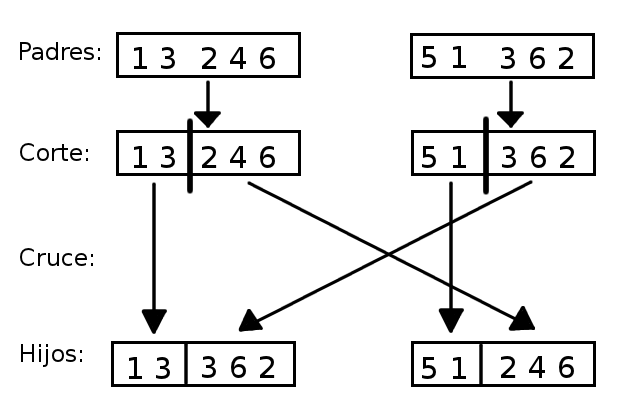
\includegraphics[width=0.5\textwidth]{./figures/cruce.png}
    \caption{Cruce de un punto}
    \label{gen: point}
\end{figure}
\item {\bf De dos puntos:} Se lleva a cabo el mismo procedimiento del cruce de
un punto, pero con dos puntos de corte. De esta misma forma, se pueden extender
a más puntos de corte.
\end{itemize}

\item {\bf Mutación:}
Consiste en modificar uno de los cromosomas bien sea de la población
o uno de los hijos generados.
\end{itemize}

\subsection{Optimizador de Enjambre de Partículas (\emph{PSO})}
    Un optimizador de enjambre de partículas (\emph{PSO}: Particle Swarm Optimizer)
es un algoritmo basado en población de optimización estocástico modelado a
partir de la simulación del comportamiento social de las bandadas de aves\cite{PSO_1}\cite{PSO_2}.

    En un sistema \emph{PSO}, un enjambre (\emph{swarm}) de partículas se mueve a
través de un espacio de búsqueda. Cada partícula representa una solución
candidata al problema de optimización. La posición de cada partícula es
influenciada por la mejor posición visitada por ella (su propia experiencia) y
la posición de la mejor partícula en su vecindad (la experiencia conjunta de
todas las partículas de su vecindad). Cuando la vecindad de una partícula es
el enjambre completo, la mejor posición en su vecindad se refiere a la mejor
partícula global y el algoritmo resultante es el \emph{gbest PSO} (Global Best
PSO). Por otra parte, cuando se utilizan vecindades más pequeñas, el algoritmo
generalmente se refiere al \emph{lbest PSO} (Local Best PSO) \cite{PSO_0}.

Las principales diferencias entre el \emph{PSO} y los \emph{EAs} son
\cite{PSO_0}:
\begin{itemize}
    \item El \emph{PSO} se ve influenciado más en la experiencia social que en la
supervivencia del más apto, como ocurren el los \emph{EAs}.
    \item En el \emph{PSO}, cada individuo se ve beneficiado de su historia. Esto
no ocurre en los \emph{EAs}.
\end{itemize}

\subsubsection{Características de las partículas}

    En el \emph{PSO}, cada partícula tiene una serie de características
\cite{PSO_0}:
\begin{itemize}
    \item $x_i(t)$: es la posición de la partícula $i$ en la iteración $t$ del
algoritmo. Es una solución factible del problema tratado.
    \item $v_i(t)$: es la velocidad de la la partícula $i$ en la iteración $t$
del algoritmo.
    \item $y_i(t)$: es la mejor posición de la partícula $i$ en la iteración $t$.
Es la mejor solución que ha tenido la partícula $i$. La elección de $y_i(t+1)$
es de la siguiente forma:

\begin{equation}\label{pso: yi}
      y_i(t+1) =
      \begin{cases}
        y_i(t)   & \text{si } f(x_i(t+1)) \geq f(y_i(t)) \\
        x_i(t+1) & \text{si } f(x_i(t+1)) < f(y_i(t))
      \end{cases}
\end{equation}
donde $f(\cdot)$ es una función de \emph{fitness} y el problema de optimización
es de minimización.
    \item $\hat{y}_i(t)$: es la mejor posición de una partícula en la vecindad de
la partícula $i$ para la iteración $t$ del algoritmo. La elección de $\hat{y}_i$
para la iteración $t + 1$ es similar a la de $y_i$:
\begin{equation}\label{pso: hatyi}
    \hat{y}_i(t + 1) = \displaystyle\min_{j \in V_k} y_j(t)
\end{equation}
donde $V_k$ es la vecindad $k$, la partícula $i$ pertenece a $V_k$ y el
problema de optimización es de minimización.

    Si sólo existe una vecindad y todas las partículas están en él, se calcula
la mejor posición de una partícula en el enjambre de partículas $\hat{y}$:
\begin{equation}\label{pso: haty}
    \hat{y}(t + 1) = \displaystyle\min_{j = 1}^{I} y_j(t)
\end{equation}
donde $I$ es la cantidad total de partículas.
\end{itemize}

    Cuando todas las partículas están en la misma vecindad, el algoritmo se
llama \emph{Global Best PSO} (\emph{gbest PSO}). Cuando las partículas pueden
estar en diferentes vecindades, el algoritmo se llama \emph{Local Best PSO}
(\emph{lbest PSO}).

\subsubsection{Actualización de la velocidad y la posición}\label{sect:metapso-vel}

    La actualización de la velocidad de la partícula $i$ para la iteración
$t + 1$ del algoritmo \emph{PSO} es \cite{PSO_0}:
\begin{equation}\label{pso: vi}
v_{i,j}(t + 1) = w \cdot v_{i,j}(t) + c_1 \cdot r_{1,j}(t) \cdot (y_{i,j}(t) - x_{i,j}(t)) + c_2 \cdot r_{2,j}(t) \cdot (\hat{y}_j(t) - x_{i,j}(t))
\end{equation}
donde,
\begin{itemize}
    \item $M$: es la cantidad de componentes para el vector velocidad de la
partícula, donde $j \in {1, \cdots, M}$
    \item $w$: es el \emph{peso inercial}, que controla el impacto que tiene la
velocidad anterior sobre la velocidad actual. Una alta inercia favorece la
exploración y una baja inercia, la intensificación.
    \item $c_1$: Es un \emph{factor de aprendizaje cognitivo} que controla a la
\emph{componente cognitiva}. Representa la atracción que una partícula tiene
hacia su éxito propio.
    \item $c_2$: Es un \emph{factor de aprendizaje social} que controla a la
\emph{componente social}. Representa la atracción que una partícula tiene hacia
éxito de sus vecinos.
    \item $r_{1,j}(t)$ y $r_{2,j}(t)$: son valores aleatorios que pertenecen al
intervalo [0, 1].
\end{itemize}

    Según Van den Bergh\cite{PSO_3}, la relación entre el \emph{peso inercial} y
las \emph{constantes de aceleración} debe satisfacer la siguiente ecuación de
modo que se garantice convergencia:
\begin{equation}\label{pso: convergece}
\displaystyle\frac{c_1 + c_2}{2} - 1 < w
\end{equation}
sino el \emph{PSO} mostraría un comportamiento acíclico o divergente.

    La actualización de la posición de la partícula $i$ para la iteración
$t + 1$ del algoritmo es de la siguiente forma \cite{PSO_0}:
\begin{equation}\label{pso: xi}
x_i(t + 1) = x_i(t) + v_i(t + 1)
\end{equation}

\subsubsection{Algoritmo general}

    Finalmente, el algoritmo general del \emph{PSO} es como se muestra en el
pseudo-código \ref{PSO}.
\begin{lstlisting}[float=h, caption=Algoritmo General PSO\cite{PSO_0}, label=PSO]
- Para cada partícula $i \in  \{1, \cdots, I\}$:
    - Inicializar $x_i$.
    //Puede ser inicializado con velocidad cero.
    - Inicializar $v_i$.
    - $y_i = x_i$.
  Fin.
- Mientras no se cumpla la condición de parada:
    - Para cada partícula $i \in \{1, \cdots, I\}$:
        - Evaluar el %\emph{fitness}% de la partícula $i$, $f(x_i)$.
        - Actualizar $y_i$ con la ecuación %(\ref{pso: yi})%.
        - Si es %\emph{gbest PSO}%:
            - Actualizar $\hat{y}$ con la ecuación %(\ref{pso: haty})%.
          Sino:
            - Actualizar $\hat{y}_i$ con la ecuación %(\ref{pso: hatyi})%.
          Fin.
        - Para cada dimensión $j \in \{1, \cdots, M\}$:
            - Actualizar velocidad $v_{i,j}$ con la ecuación %(\ref{pso: vi})%.
          Fin.
        - Actualizar posición $x_i$ con la ecuación con la ecuación %(\ref{pso: xi})%.
      Fin.
  Fin.
\end{lstlisting}

\subsection{Evolución Diferencial (\emph{DE})} \label{sect:metade}

    Es un algoritmo basado en población que hace uso de
una representación de punto flotante (codificación real) y bastante parecido al
genético. Tiene los operadores de cruce y selección, pero no mutación. Su
funcionamiento según \cite{SwAjAm2008} es el siguiente:

    El $i$-ésimo vector individuo (cromosoma) de la población con tiempo
(generación) $t$ tiene $s$ componentes:
%Ejemplo de vector.
%INICIO
\begin{equation} \label{de: vector}
    \overrightarrow{Z_i}(t) = [ Z_{i,1}(t), Z_{i,2}(t), \cdots, Z_{i,s}(t) ]
\end{equation}
%END

    Para cada vector individuo $\overrightarrow{Z_i}(t)$ perteneciente a la
generación $t$ de la población, se toman aleatoriamente a tres individuos
$\overrightarrow{Z_j}(t)$, $\overrightarrow{Z_k}(t)$ y $\overrightarrow{Z_m}(t)$,
de modo que se cumpla $i \neq j \neq k \neq m$. Se genera entonces al hijo
$\overrightarrow{U_i}(t + 1)$ de la siguiente forma:
\begin{equation} \label{de: crossover}
 \forall n \in [1, s]\text{; }U_{i,n}(t+1) =
 \begin{cases}
   Z_{m,n}(t) + \gamma \cdot (Z_{j,n}(t) - Z_{k,n}(t))  & \text{si } rand(0,1) < Cr\\
   Z_{i,n}(t)                               & \text{cualquier otro caso}
 \end{cases}
\end{equation}
donde $Cr \in [0, 1]$ es la tasa de cruce y $\gamma \in [0, 1]$. Si el
hijo $\overrightarrow{U_i}(t + 1)$ tiene mejor valor de función de \emph{fitness},
entonces reemplaza al padre $\overrightarrow{Z_i}(t)$ en la siguiente generación,
sino el padre permanece en la siguiente generación y el hijo se descarta:
\begin{equation} 
  \overrightarrow{Z_i}(t+1) =
  \begin{cases}
    \overrightarrow{U_i}(t+1) & \text{si } f(\overrightarrow{U_i}(t+1)) < f(\overrightarrow{Z_i}(t)) \\
    \overrightarrow{Z_i}(t)   & \text{si } f(\overrightarrow{U_i}(t+1)) \geq f(\overrightarrow{Z_i}(t))
  \end{cases}
\end{equation}
donde $f(\cdot)$ es una función de \emph{fitness} para un problema de
optimización de minimización.

    El algoritmo general del \emph{DE} se muestra en el pseudo-código \ref{DE}.
\begin{lstlisting}[float=h, caption=Algoritmo General DE \cite{SwAjAm2008}, label=DE]
- Inicializar y evaluar funciones %\emph{fitness}% de cada
  individuo $i \in  \{1, \cdots, I\}$.
- Mientras no se cumpla la condición de parada:
    - Para cada individuo $i \in \{1, \cdots, I\}$:
        - Elegir tres individuos aleatorios $j$, $k$, $m$.
        - Generar hijo %$\overrightarrow{U_i}$% aplicando la ecuación (%\ref{de: crossover}%).
        - Si $f(\overrightarrow{U_i})$ < $f(\overrightarrow{Z_i})$:
            - Reemplazar %$\overrightarrow{Z_i}$% por %$\overrightarrow{U_i}$%.
          Fin.
      Fin.
  Fin.
\end{lstlisting}

\subsection{Algoritmo de Abeja (\emph{Bee})} \label{sect:metabee}

    El algoritmo de Abeja (\emph{Bee}) es un algoritmo poblacional de
optimización estocástico mo\-de\-la\-do a partir de la simulación del comportamiento
social y habilidades de búsqueda de las colonias de abejas mieleras \cite{BEE_0}.

\subsubsection{Abejas en la naturaleza}

    Una colonia de abejas mieleras puede extenderse largas distancias
de modo que se exploten grandes números de fuentes de comida al mismo
tiempo. Este proceso comienza en una colonia con abejas exploradoras
que son enviadas a los sitios de flores más prometedores. Los sitios
prometedores son aquellos con grandes cantidades de néctar o polen
que pueden ser recolectados con menos esfuerzo. Estos sitios tienden a ser
visitados por más  abejas, mientras que los sitios con menor calidad tienden
a ser menos visitados \cite{BEE_0}.

    Durante la época de cosecha, una colonia continúa su exploración
manteniendo un porcentaje de la población como abejas exploradoras.
Cuando retornan a la colmena, esas abejas exploradoras depositan el
polen o néctar y van al \emph{piso de la danza} a ejecutar un baile
conocido como \emph{danza oscilante}. Esta es esencial para la comunicación
en la colonia y contiene tres piezas de información
de cada uno de los sitios visitados \cite{BEE_0}: 
\begin{itemize}
    \item La dirección hacia donde está el sitio.
    \item La distancia desde la colonia.
    \item Su calidad (\emph{fitness}).
\end{itemize}
    Esta información, ayuda a la colonia a enviar sus abejas a los sitios de
flores de manera más precisa, sin usar guías o mapas \cite{BEE_0}.

    Después de la \emph{danza oscilante}, las abejas exploradoras van a los
sitios que encontraron con abejas que estaban esperando dentro de la colmena.
Más seguidoras son enviadas a los mejores sitios. Esto le permite a la colonia
recolectar comida más rápido y eficientemente \cite{BEE_0}.

    Mientras recolectan comida de un sitio, las abejas monitorizan su nivel de
comida. Esto es necesario para decidir cuando ocurrirá la siguiente
\emph{danza oscilante}\cite{BEE_0}.

\subsubsection{Abejas en el algoritmo}

    En el \emph{Bee}, cada abeja tiene una solución al problema de optimización
(sitio de flores) y la función de \emph{fitness} (calidad del sitio) asociada a
ella \cite{BEE_0}.

    El algoritmo depende de los siguientes parámetros \cite{BEE_0}:
\begin{itemize}
    \item $m$: Cantidad de sitios de flores disponibles en cada iteración.
Cada sitio de flores es una solución factible al problema de optimización y
cada abeja tiene la dirección hacia un sitio de flores.
    \item $e$: Cantidad de sitios de flores élite. Son los $e$ mejores sitios de
flores encontrados por las abejas.
    \item $eb$: Cantidad de abejas élite. Esta será la cantidad de abejas que
serán enviadas a los mejores sitios de flores.
    \item $ob$: Cantidad de abejas exploradoras. Estas abejas serán asignadas a
buscar nuevos sitios de flores (nuevas soluciones).
    \item $I$: Cantidad de abejas de la colmena.
\end{itemize}

    El algoritmo entonces consiste en emular lo que ocurre en la naturaleza al
elegir los $e$ mejores sitios de flores y asignar a cada abeja a un sitio
dependiendo de su calidad. Luego, todas las abejas harían una búsqueda en
vecindad para encontrar nuevas soluciones. El proceso se repite una y otra vez
hasta que la condición de parada se cumpla \cite{BEE_0}.

    El algoritmo general de Abeja se muestra en el pseudo-código \ref{Bee}.
\begin{lstlisting}[float=h, caption=Algoritmo General de Abeja\cite{BEE_0}, label=Bee]
- Para cada abeja $i \in  \{1, \cdots, I\}$:
    - Inicializar los sitios de flores de cada abeja.
    - Evaluar función de %\emph{fitness}% de cada abeja.
  Fin.
- Mientras no se cumpla la condición de parada:
    - Seleccionar los mejores sitios. //%\color{darkgrey}\emph{Danza Oscilante}%
    - Asignar $e$ abejas a los mejores sitios.
    - Asignar $m - e$ abejas sitios aleatorios.
    - Para cada abeja $i \in \{1, \cdots, I\}$:
        - Hacer búsqueda en la vencindad del sitio asignado.
        - Evaluar el %\emph{fitness}% de cada nuevo sitio.
    Fin.
  Fin.
\end{lstlisting}

\subsection{Algoritmo de Hormiga (Ant)}
\label{sect:metaant}

    Existen varias metaheurísticas usadas para resolver problemas combinatorios
difíciles, ins\-pi\-ra\-das en diversos comportamientos de las hormigas:
\begin{itemize}
    \item \textbf{Optimización de Colonias de Hormigas (\emph{ACO})}: está basada
en los rastros de fer\-or\-mo\-na que dejan las hormigas por donde caminan cuando
están en búsqueda de comida. Esto lo hacen para ``construir'' un camino que sus
compañeras puedan seguir. Las ferormonas se evaporan con el tiempo, de modo que
un camino poco usado se terminará desvaneciendo. Los caminos más transitados,
normalmente llevan a las hormigas a fuentes de alimento abundantes de manera
eficiente. En el algoritmo propuesto por Marco Dorigo en 1992 \cite{Ant_0}, los
caminos más usados por las hormigas, representan a las mejores soluciones del
problema tratado.
    \item \textbf{Algoritmo de \emph{Clustering} de Hormigas (\emph{ACA})}\cite{OuBa2007}: es
un algoritmo basado en cómo las hormigas organizan los cadáveres de sus
compañeras dentro de su colonia, simulando un cementerio. En el algoritmo, las
hormigas se mueven en un espacio de dos dimensiones o \emph{grid}. El deber de
cada hormiga es cargar un cadáver y llevarlo a la pila de cadáveres donde
debería ir.
\end{itemize}
